\chapter{نتایج جدید}
\label{chapter:results}
در این فصل ابتدا به بررسی مقاله
\cite{arya}
 می‌پردازیم. این مقاله پایه تحقیقاتی نتایج جدید به دست آمده در این پایان‌نامه است. مزومدار در این مقاله با تعریف مسئله‌ی
\transf{سیستم ذخیره‌سازی توزیع شده با قابلیت بازیابی محلی تک-شکست}{single-failure locally recoverable distributed storage system}
اثبات می‌کند این مسئله‌ی دوگان مسئله‌ی کدگذاری اندیس است.

بعد از بررسی کار مزومدار با تعمیم مسئله‌ی سیستم ذخیره‌سازی و معرفی مسئله‌ی
\transf{کدگذاری منبع انعطاف پذیر}{PSIC: Pliable source index coding}
 اثبات می‌کنیم، این مسئله‌ی تعمیم یافته، دوگان 
 \picod
  در حالت خطی است.
\newpage

\section{
 سیستم ذخیره‌سازی توزیع شده با قابلیت بازیابی محلی تک-شکست
}
یکی از چالش‌ها در سیستم‌های ذخیره سازی داده توزیع شده، بازیابی داده‌های از دست رفته به دلیل خراب شدن یکی از سرورها است. 
برای حل این مشکل هر داده در چندین سرور ذخیره می‌شود تا در صورت از بین رفتن یکی از سرورها داده‌های آن سرور از دست نرود. چالش این روش هزینه‌ی بازیابی سرور از دست رفته است. یعنی زمانی که سرور خراب شده را جایگزین می‌کنیم و قصد داریم داده‌های سرور قبلی را روی سرور جدید قرار دهیم باید آن داده‌ها را از بقیه سرورهای شبکه 
\transf{دریافت}{download}
کنیم. اما هزینه‌ی دریافت یک داده از سرورهای مختلف متفاوت است.
``در سیستم‌های توزیع شده خراب شدن یک تک سرور متداول ترین مشکل است.``

``مطالعه‌ی سیستم‌های ذخیره سازی با قابلیت بازیابی اولین بار در
\cite{5550492}
مورد توجه قرار گرفت. در چندین کار جدید این مسیر ادامه پیدا کرد. در
\cite{6259860}
توصیف مرتبی برای
\transf{ویژگی بازیابی محلی}{locally repairable property}
ارائه می‌شود. نتایج این مقاله در جهت‌های مختلف توسعه داده شده است و حتی نتایجی از جنس غیرممکن بودن نیز کشف شده است (برای مثال به
\cite{6570829, kamath2013codes,6818438,silberstein2013optimal, tamo2013optimal}
و به خصوص مقاله اخیر 
\cite{Tamo_2014}
رجوع کنید.). نکته قابل توجه در مقالات بالا عدم توجه به توپولوژی شبکه است و به تمام سرور ها بدون در نظر گرفتن محل فیزیکی آن‌ها، نزدیکی به هم دیگر و ارتباطاتشان با بقیه سرورها نگاه می‌شود.
 ``
 
 مزومدار در ادامه از یک گراف برای در نظر گرفتن توپولوژي واقعی شبکه استفاده می‌کند. هر راس متناظر یک سرور است و هر دو سروری که با هم ارتباط دارند با یک یال به یک دیگر متصل شده اند. سپس اثبات می‌کند این مدل جدید دوگان مسئله کدگذاری اندیس است.
 
 \subsection{
 برابری 
 \icod
  و ظرفیت سیستم ذخیره‌سازی توزیع شده با قابلیت بازیابی محلی تک-شکست
 }
\label{subsec:arya}
 شبکه‌ی ارتباطی یک سیستم ذخیره سازی توزیع شده را در نظر بگیرید.
 \autoref{fig:storage-graph}
 یک مثال برای چنین شبکه‌ای است. ارتباط بین سرورها بر اساس توانایی ارتباطی آن‌ها است(که می‌تواند به خاطر فاصله‌ی جغرافیایی ارتباطات فیبر نوری و \ldots). همچنین ممکن است به خاطر مسائل فنی در تفاوت فنی میان سرورها و ارتباطشان(مثال سرعت متفاوت دانلود و آپلود) از گراف جهت دار استفاده کنیم.
 
 هدف ما این است که اگر یکی از سرورها دچار مشکل شود و دیتای آن از بین برود سرور جایگزین شده در همان نقطه بتواند با گرفتن اطلاعات از سرورهایی که به این نقطه وصل هستند دیتای سرور از دست رفته را بازیابی کند.
 
 سوال ما این است که با داشتن شبکه‌ی سرورها بیشترین مقدار اطلاعاتی که می‌توان در شبکه ذخیره کرد چقدر است؟
\begin{figure}[H]
	\centering
	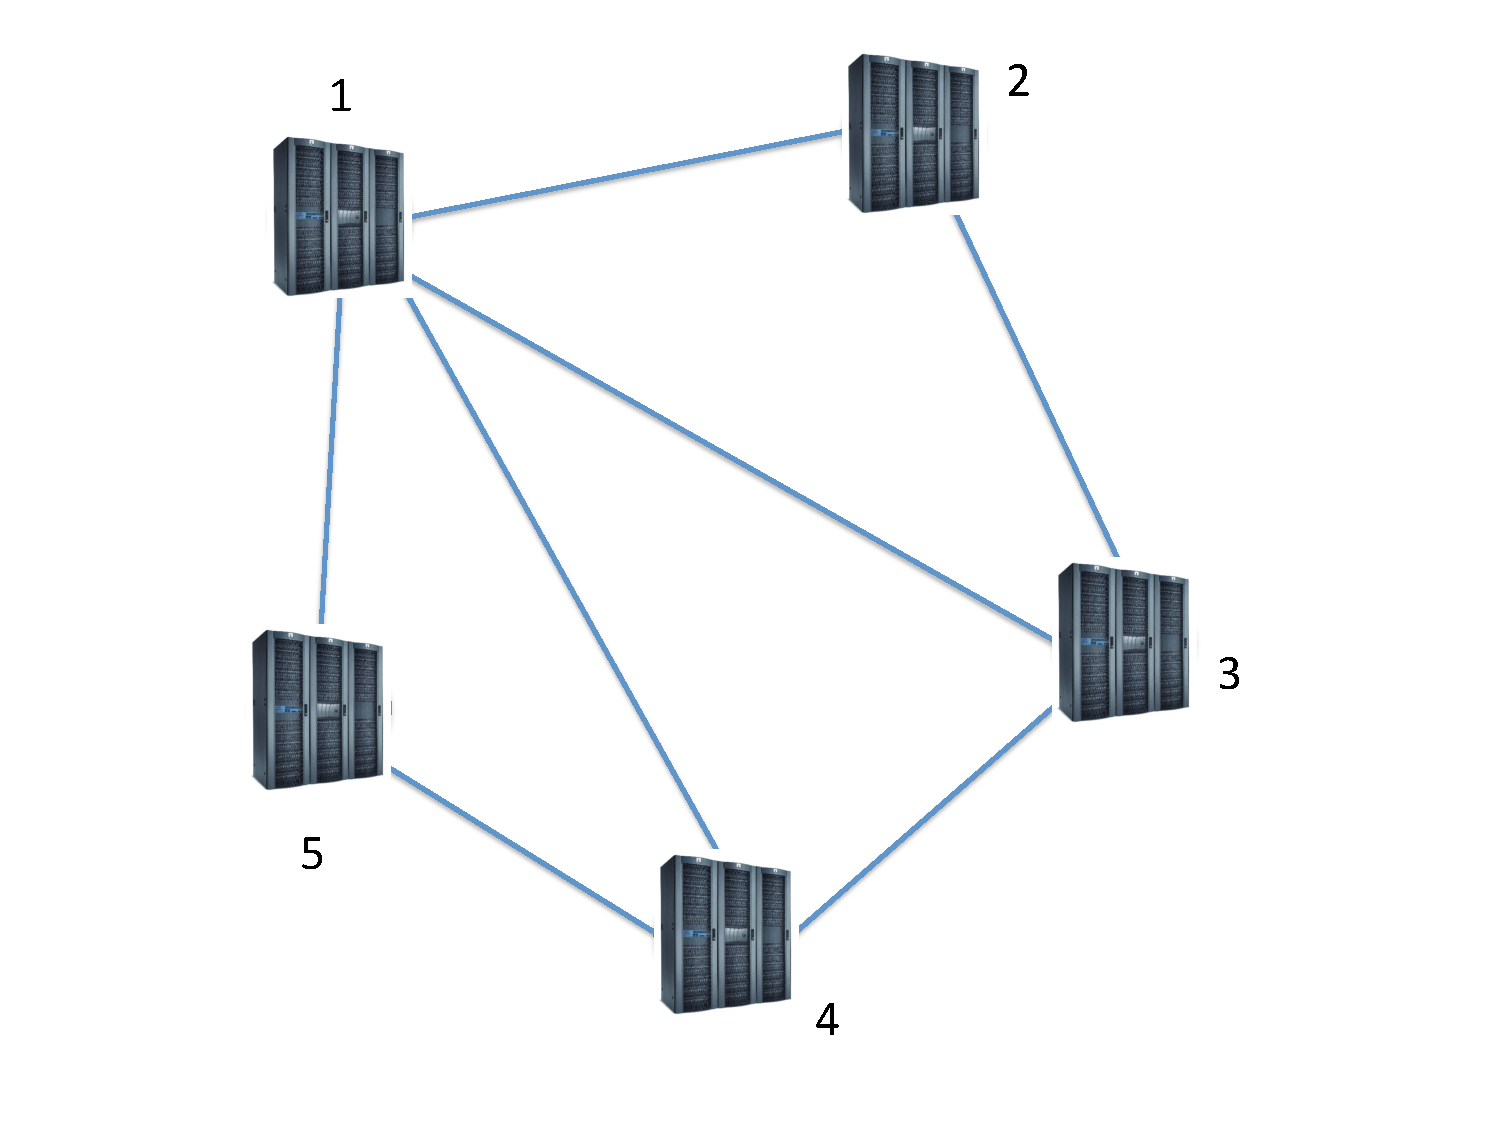
\includegraphics[width=0.5\linewidth]{figs/chapter6/storage-graph}
	\caption[
	مثالی از یک شبکه ارتباطی سرورهای یک سیستم ذخیره‌سازی توزیع شده]{
		مثالی از یک شبکه ارتباطی سرورهای یک سیستم ذخیره‌سازی توزیع شده
		\cite{arya}
		}
	\label{fig:storage-graph}
\end{figure}

\begin{definition}[\transf{کد ذخیره سازی توزیع شده قابل بازیابی}{RDSS-code}]
	برای گراف جهت‌دار
	$G(V, E)$
	که
	$V = [n]$
	میدان
	$\mathbb{F}_{q}$
	و متغیرهای تصادفی
	$X_1, X_2, \ldots, X_n \in \mathbb{F}_{q}$
		کد ذخیره سازی توزیع شده قابل بازیابی 
		$\mathcal{C} \subseteq \mathbb{F}_{q}$
		،  مجموعه‌ای از بردار‌ها از
		$\mathbb{F}_{q}$
		همراه با مجموعه‌ی توابع قطعی بازیابی به شکل
		$f_i: \mathbb{F}_q^{|N(i)|} \to \mathbb{F}_q$
		است به طوری که برای هر مجموعه از متغیرهای تصادفی 
		$(X_1, X_2,\dots,X_n) \in \mathbb{F}_q^n$
		داشته باشیم:
		$$X_i = f_i(\{X_j: j \in N(i)\}), \quad i = 1,\dots,n$$
\end{definition}

به
$\log_q(|C|)$
\transf{بعد کد}{dimension of code}
 گفته می‌شود. برای گراف داده شده‌ی $G$ بزرگترین بعد کد را با
 $RDSS_q(G)$
 نشان می‌دهیم.
  \begin{definition}
  	میگوییم ماتریس
  	$A_{n \times n} = (a_{ij}), a_{ij} \in \mathbb{F}_q$
  	بر گراف
  	$G(V, E)$
  	\transf{مطابقت}{fits}
  	می‌کند اگر 
  	\begin{latin}
  		\begin{align*}
  			& \forall i : a_{ii} \ne 0 \\
  			& \forall i \ne j:  (i, j) \notin E \Rightarrow a_{ij} = 0
  		\end{align*}
  	\end{latin}
  \end{definition}
 \begin{definition}[\transf{رتبه کمینه}{minrank}]
	 \label{def:minrank}
 	رتبه کمینه گراف
 	$G$
 	بر روی میدان
 	$\mathbb{F}_q$
 	به صورت زیر تعریف می‌شود:
 	\begin{equation}
 		\minrank_q(G) = \min\{\rank_{\mathbb{F}_q}(A): A \text{ fits } G\}.
 	\end{equation}
 \end{definition}
 \begin{theorem}
	 \label{thm:minranl}
 	در
 	\cite{4031356}
 	نشان داده شده است که:
 	\begin{equation}
 		\indx_q(G) \le \minrank_q(G),
 		\label{eq:bary}
 	\end{equation} 
 \end{theorem}
 \begin{example}[
 	توابع خطی
 	\cite{arya}
 	]

 	برای گراف داده شده در
 	\autoref{fig:storage-graph}
 	داریم:
 	$
 		N(1) = \{2,3,4,5\}, \, N(2)  = \{1,3\}, N(3)  = \{1,2,4\}, N(4)  = \{1,3,5\},  N(5)  = \{1,4\}
 	$.
 	اگر داده‌ی درون سرور
 	$i$
 	را با
 	$X_i$
 	نشان دهیم برای این‌که بتوانیم در صورت از دست رفتن یک سرور اطلاعات آن را به صورت محلی بازیابی کنیم باید توابع زیر را داشته باشیم:
 	$X_1 = f_1(X_2,X_3,X_4,X_5), X_2 = f_2(X_1,X_3), X_3 = f_3(X_1,X_2,X_4), X_4 = f_4(X_1,X_3, X_5), X_5 = f_5(X_1, X_4)$.

 	فرض کنید توابع
 	$f_i$
 	همگی خطی هستند پس برای
 	$\alpha_{ij} \in  \mathbb{F}_q, 1\le i,j\le 5,$
 	خواهیم داشت:
 	 	\begin{align*}
 		X_1 &= \alpha_{12} X_2 +\alpha_{13} X_3 + \alpha_{14}X_4 + \alpha_{15}X_5\\
 		X_2 &= \alpha_{21}X_1+\alpha_{23}X_3\\
 		X_3 &= \alpha_{31}X_1 +\alpha_{32}X_2+\alpha_{34}X_4\\
 		X_4 &= \alpha_{41}X_1 + \alpha_{43}X_3 + \alpha_{45}X_5\\
 		X_5 &= \alpha_{51}X_1+\alpha_{54}X_4.
 	\end{align*}
 	که نتیجه خواهد داد که
 	$(X_1,X_2,\dots, X_5)$
 	در فضای پوچ ماتریس
 	\[
 	D \equiv
 	\left( \begin{array}{ccccc}
 		1 & -\alpha_{12} & -\alpha_{13}  & - \alpha_{14} & -\alpha_{15} \\
 		-\alpha_{21} & 1 &  -\alpha_{23} & 0 & 0 \\
 		-\alpha_{31} & -\alpha_{32} & 1 & -\alpha_{34} & 0\\
 		-\alpha_{41} & 0 &-\alpha_{43}  & 1 & -\alpha_{45}\\
 		-\alpha_{51} &0 & 0 & -\alpha_{54} & 1
 	\end{array} \right).\] 
 	قرار دارد.
 	
 	بعد فضای پوچ ماتریس برابر
 	$|null(D)| = n - rank(D)$
 	است. پس اگر خود را به توابع خطی محدود کنیم خواهیم داشت:
 	$$RDSS_q(G) = n - minrank_q(G)$$
 	ولی برای توابع غیر خطی این تساوی برقرار نخواهد بود و خواهیم داشت:
 	\begin{equation}
 		\rdss_q(G) \ge n - \minrank_q(G),
 		\label{eq:minrk}
 	\end{equation}
 	این نامساوی و نامساوی
 	\autoref{eq:bary}
 	این حدس را به ما میدهد که
 	$\rdss_q(G) = n - \indx_q(G)$
 	ولی متاسفانه همان‌طور که در مثال بعدی می‌بینیم این حدس درست نیست.
 \end{example}
 
 \begin{example}[
 	تاثیر توابع غیر خطی
 	\cite{arya}
 	]
 	گراف زیر را در نظر بگیرید:
\begin{figure}[H]
	\centering
	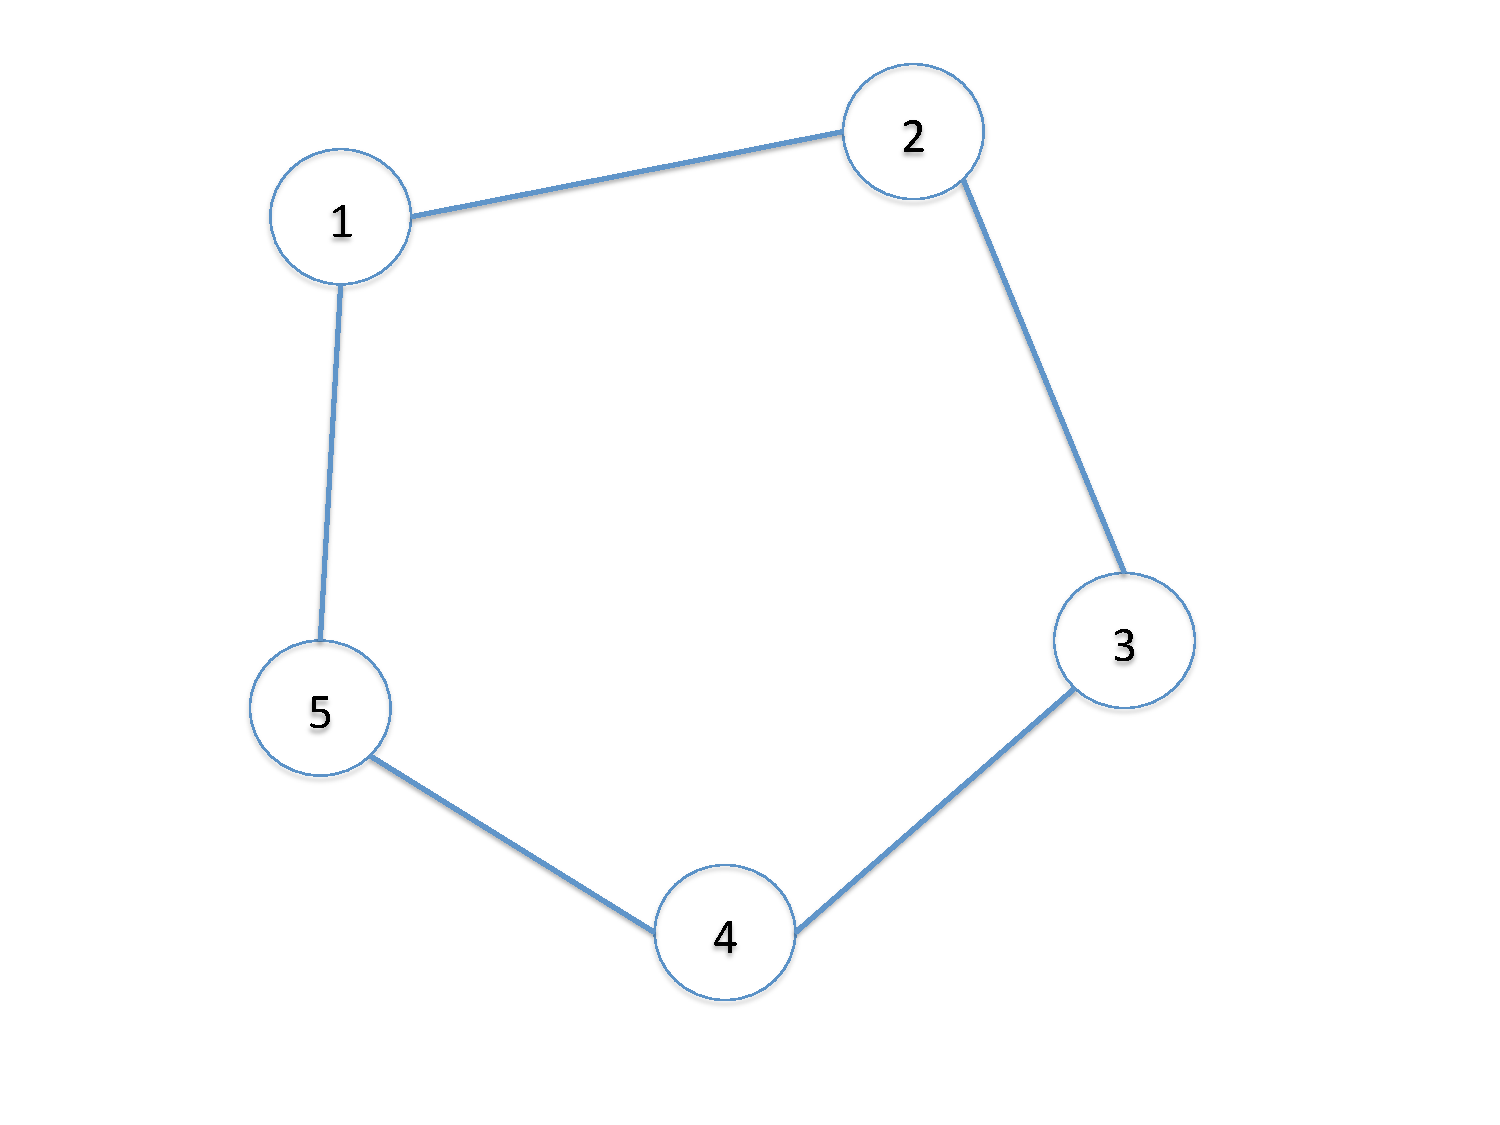
\includegraphics[width=0.7\linewidth]{figs/chapter6/storage-graph-pent}
	\caption[مثال تاثیر توابع غیر خطی]{
		مثال تاثیر توابع غیر خطی
	\cite{arya}
	}
	\label{fig:storage-graph-pent}
\end{figure}
بزرگترین کد برای این گراف به شکل زیر است:
$\{00000,01100,00011,11011,11101\}$
که توابع مربوطه به شکل زیر خواهد بود:
\begin{align*}
	X_1 = X_2 \wedge X_5, 
	X_2 = X_1 \vee X_3,
	X_3 = X_2 \wedge \bar{X}_4, \\
	X_4 = \bar{X}_3 \wedge X_5
	X_5 = X_1\vee X_4.
\end{align*}
که نتیجه می‌دهد:
$\rdss_2(G) = \log_2 5$
ولی میدانیم که
$\indx_2(G)=3$.
زیرا اگر فرستند مقادیر
 $Y_1= X_2+X_3, Y_2= X_4+X_5$ 
 و
  $Y_3= X_1+X_2+X_3+X_4+X_5.$
  را ارسال کند گیرنده‌ها می‌توانند با توابع
  $X_1 = Y_1 + Y_2+Y_3; X_2 = Y_1+X_3; X_3 = Y_1+X_2; X_4 = Y_2+X_5; X_5 = Y_2+X_4.$
  پیام‌های خود را بازیابی کنند.
 \end{example}
 
 با وجود آنکه در حالت کلی 
 $\rdss_q(G) \ne n - \indx_q(G)$
 ولی این دو مقدار فاصله‌ی زیادی از هم ندارند. بلکه برای الفباهای با اندازه به اندازه‌ی کافی بزرگ می‌توان آن‌ها را به اندازه‌ی دلخواه به هم نزدیک کرد. این نکته از 
 \autoref{thm:aryamain}
 نتیجه می‌شود.
 \begin{theorem}\label{thm:aryamain}
 	برای گراف
 	 $G(V,E)$,
 	 داریم
 	\begin{align}
 		n - \rdss_q(G) \le \indx_q(G) \le n -\rdss_q(G) + \log_q\Big(\min\{n\ln q, 1+ \rdss_q(G)\ln q \}\Big). 
 	\end{align}
 \end{theorem}
 
 این قضیه در
 \cite{4691014}
 با ابزار های نظریه‌ی گراف اثبات می‌شود . مزومدار در ادامه با اثباتی الگوریتمی این قضیه ثابت می‌کند. از آنجایی که اثبات این قضیه کاربردی در نتایج جدید ما ندارد از تکرار آن پرهیز می‌کنیم.

 
\section{نتایج جدید}
\label{sec3}
\subsection{
	برابری 
	\picod
	 و کدگذاری منبع منعطف
}
در این بخش، ابتدا به طور رسمی مسئله کدگذاری منبع انعطاف پذیر را تعریف می‌کنیم. سپس، قضیه اصلی این مقاله را در مورد ارتباط بین مسئله 
\picod
 و کد منبع انعطاف پذیر خطی بیان می‌کنیم.
\subsubsection{
		کدگذاری منبع انعطاف پذیر
}
\begin{recal}
	دلیل این‌که از واژه‌ی اندیس در نام‌گذاری مسئله کدگذاری اندیس استفاده شده است این است که می‌توان نگاه متفاوتی به مسئله داشت. در نگاه اول مسئله شامل یک فرستنده و تعدادی گیرنده است که گیرنده‌ها به دنبال داده‌ی جدیدی هستند و وظیفه‌ی فرستنده است که با ارسال پیام‌هایی آن‌ها را آگاه کند. اما نگاه دیگری نیز وجود دارد. در نگاه قبل ما دو عنصر اصلی در مسئله داشتیم: فرستنده و گیرنده‌ها(و البته اطلاعات جانبی گیرنده‌ها). ولی می‌توان خود پیام‌ها را هم به عنوان یک عنصر اصلی در مسئله دید.
	
فرض کنید 
$n$
پیام(متغیر‌ تصادفی) از
$\mathbb{F}_q$
 داریم. قبل از مشخص شدن پیام‌ها، فرستنده و گیرنده‌ها تعدادی مجموعه به شکل
 $\forall i \in [k]: A_i \subseteq \fq$
 مشخص می‌کنند که اجتماع آن‌ها کل فضای پیام‌ها را پوشش دهد یعنی:
 $ \bigcup\limits_i^k A_i = \fq^n $
 و علاوه بر آن اگر هر گیرنده بداند پیام‌ها در کدام
 $A_i$
 است بتواند بر اساس اطلاعات جانبی خود پیام مورد نظر خود را بازیابی کند. سپس بعد از مشخص شدن پیام‌ها، فرستنده تنها اندیس مجموعه‌ی شامل پیام را برای گیرنده‌ها ارسال کند. این کار تنها به
 $\log_q(k)$
 ارسال پیام از طرف فرستنده نیاز دارد.
\end{recal}
\begin{example}
	\cite{ourwork}
	فرض کنید پیام‌ها از
	$\mathbb{F}_2$
	می‌آیند یعنی
	$X_i \in \{0, 1\}$
	برای گراف اطلاعات جانبی زیر چند فرستنده چه پیام‌هایی می‌تواند بفرستد؟
	\newline
		\begin{minipage}{0.5\textwidth}
			
				\begin{figure}[H]
					\centering
				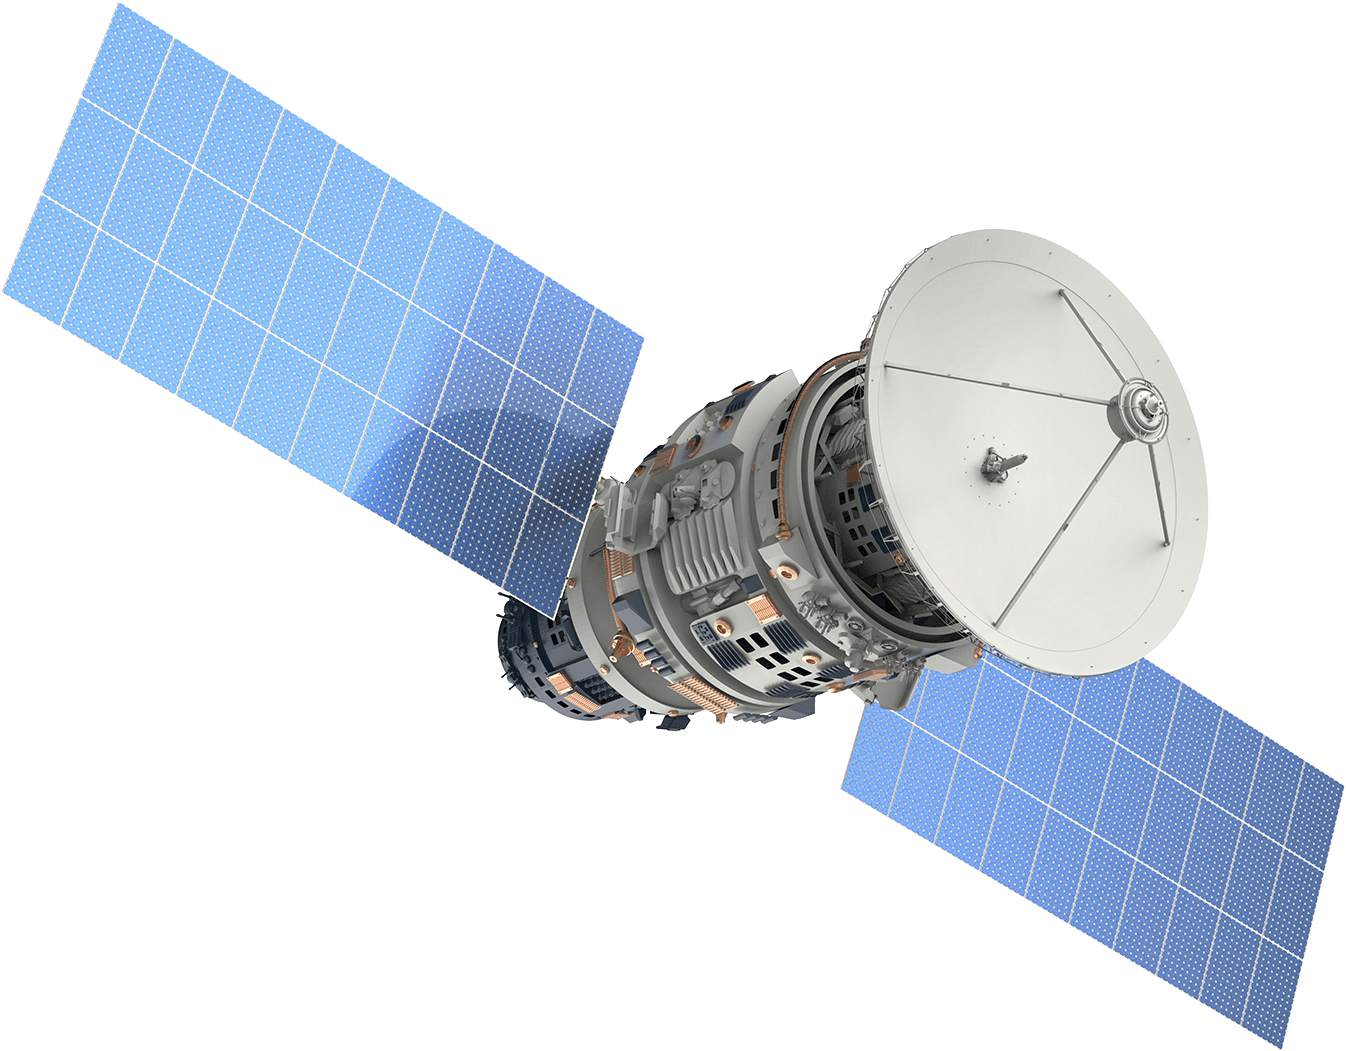
\includegraphics[width=0.3\linewidth]{figs/chapter6/satelite}
			\end{figure}
		\begin{enumerate}
		\item\centering$Y = (X_1,X_2,X_3)$
		\item \centering$Y = (X_1 + X_2 + X_3) $
\end{enumerate}
	\end{minipage}
		\begin{minipage}{0.5\textwidth}
		\centering
		\begin{tikzpicture}[->, >=stealth, auto, semithick]
			% Set the positions of the nodes
			\node[circle, draw=blue, fill=blue!20, inner sep=0pt] (C1) at (0,2) {
					
\includegraphics[width=0.06\linewidth]{figs/chapter6/thinkingemoji.png}
			};
			\node[circle, draw=blue, fill=blue!20, inner sep=0pt] (C2) at (1.5,2) {
					
\includegraphics[width=0.06\linewidth]{figs/chapter6/thinkingemoji.png}
			};
			\node[circle, draw=blue, fill=blue!20, inner sep=0pt] (C3) at (3,2) {
					
\includegraphics[width=0.06\linewidth]{figs/chapter6/thinkingemoji.png}
			};
			\node[above] at (1.5,2.5) {We want to know more};
			
			
				\node[circle, draw=green, fill=green!20, inner sep=0pt] (B1) at (0,0) {$B_1$};
				\node[circle, draw=green, fill=green!20, inner sep=0pt] (B2) at (1.5,0) {$B_2$};
				\node[circle, draw=green, fill=green!20, inner sep=0pt] (B3) at (3,0) {$B_3$};
				\node[below] at (1.5,-0.5) {messages};
			
			
				% Draw the edges
				\draw (C1) -- (B1);
			%	\draw[->, color=red]  (C1) -- (B2);
				\draw (C1) -- (B3);
				
				\draw (C2) -- (B1);
				\draw (C2) -- (B2);
			%	\draw[->, color=red]  (C2) -- (B3);
				
		%		\draw[->, color=red]  (C3) -- (B1);
				\draw (C3) -- (B2);
				\draw (C3) -- (B3);
			
			% Position the parts
			\begin{scope}[on background layer]
				\node[fit=(C1) (C2) (C3), draw=blue, fill=blue!10, rounded corners] {};
				\node[fit=(B1) (B2) (B3), draw=green, fill=green!10, rounded corners] {};
			\end{scope}
		\end{tikzpicture}			
	\end{minipage}
	\newline
		فرستنده می‌تواند در روش اول با سه ارسال نیاز تمام گیرنده‌ها را ارضا کند. در روش دوم تنها با یک ارسال این کار را انجام می‌دهد. زیرا هر گیرنده با استفاده از توابع زیر می‌تواند پیام مورد نظر خود را بازیابی کند:
	\begin{align*}
		\begin{cases}
				X_1 &= Y - X_2 - X_3 \\
				X_2 &= Y - X_1 - X_3  \\
				X_3 &= Y - X_1 - X_2  
			\end{cases}   
	\end{align*}
	با توجه به بحث بالا در مورد نحوه‌ی نگاه به مسئله می‌توان دید که در واقع فرستنده پیام‌ها را به دو دسته تقسیم می‌کند.
	\begin{latin}

		\begin{enumerate}
			\centering
			\item $\{X: X_1 + X_2 + X_3 = 1\}$
			\item $\{X: X_1 + X_2 + X_3 = 0\}$
		\end{enumerate}
	\end{latin}
	حال هر کدام از گیرنده‌ها بر اساس این‌که پیام در کدام دسته است می‌توانند پیام مورد نظر خود را بازیابی کنند.
\end{example}

همان‌طور که در مثال قبل دیدیم مسئله 
\icod
 را می‌توان به نوعی مسئله‌ی دسته بندی فضای پیام‌ها دید. بر اساس همین ایده مسئله کدگذاری منبع را تعریف می‌کنیم. در مسئله کدگذاری منبع، هیچ فرستنده‌ای وجود ندارد که به گیرنده‌ها بگوید کدام مقدار برای $X$ انتخاب شده است. به جای آن، مجموعه‌ای از بردارهای
  $\mathbb{F}^m$
   وجود دارد که به این مجموعه
\transf{کتاب کد}{code book}
 (یا 
 \transf{جدول}{table})
 گفته می‌شود که $X$به آن تعلق دارد. سپس، با توجه به اطلاعات جانبی و کتاب کد، هر گیرنده باید پیام مورد نظر خود را بازیابی کند.
\begin{observation}
	مسئله‌ی کدگذاری منبع همان مسئله‌ی کد ذخیره سازی توزیع شده قابل بازیابی است! مسئله‌ی کد ذخیره سازی را نمی توان برای حالت منعطف به صورتی تعمیم داد که هنوز معنا دار باشد. نتیجه جدید به دست آمده در این پایان‌نامه تعمیم نتیجه مزومدار برای حالت منعطف(و همچنین خطی) است.
\end{observation}

\begin{observation}
توجه داشته باشید که در مسئله 
\picod
، هدف کاهش اندازه پیام‌های منتقل شده است در حالی که در مسئله 
\psicod
، هدف افزایش اندازه کتاب کد (جدول قابل استفاده) است.
\end{observation}

\begin{definition}[جدول قابل استفاده]
	\label{def1}
برای یک الفبای داده شده
 $\mathbb{F}$
  و گراف اطلاعات جانبی 
 $G$، 
 یک جدول قابل استفاده 
 $T$
  زیرمجموعه‌ای از 
 $\mathbb{F}^m$ 
 است به طوری که برای هر گیرنده 
 $c_i$
 حداقل یک شاخص 
  $j \in R_i$
  وجود دارد که به ازای تمام اعضای
  $T$
  که با اطلاعات جانبی
  $c_i$
  تطبیق دارند در عضو
  $j$
  ام یکسان باشند. یعنی:
\begin{align*}
    \forall i: \exists j \notin S_i: \forall X, X^\prime: X[S_i] = {X^\prime}[S_i]  \Rightarrow X[j] = {X^\prime}[j]
\end{align*}
ما از اصطلاح جدول استفاده می‌کنیم زیرا عناصر این مجموعه را در یک جدول نمایش می‌دهیم. به این ترتیب، هر ستون یکی از متغیرهای $X_i$ را نشان می‌دهد و هر سطر یک پیام ممکن است.
\end{definition}

مسئله کدگذاری منبع انعطاف‌پذیر، 
\psicod
، برای یافتن بزرگترین جدول قابل استفاده ممکن برای یک $G$ داده شده است.

\begin{remark}
    ما همیشه می‌توانیم
     $\mathbb{F}^n$ 
     را به جدول‌های قابل استفاده تقسیم کنیم، به عنوان مثال هر 
     $x \in \mathbb{F}^n$ 
     را به عنوان یک جدول قابل استفاده با یک ردیف در نظر بگیریم.
\end{remark}

\begin{lemma}
    برای گراف $G$ و جدول‌های قابل استفاده‌ی
    $T_1, \ldots, T_l \subseteq \mathbb{F}^m$
     که
     $\bigcup\limits_{i} T_i =  \mathbb{F}^m$
     ، یک راه‌حل برای
     \picod
     وجود دارد که تابع رمزگذاری آن عبارت است از تابعی که اندیس جدول قابل استفاده‌ای را ارسال می‌کند که متغیرها از آن انتخاب شده اند.
\end{lemma}
\begin{proof}
    گیرنده $c_i$ را در نظر بگیرید. گیرنده 
    $c_i$
    ،
    $X[S_i]$
    را به عنوان اطلاعات جانبی خود دارد. بر اساس تعریف جدول قابل استفاده، شاخص 
    $j \in R_i$
     وجود دارد که
      $c_i$ 
      می‌تواند
      $x_j$
      را بازیابی کند.
\end{proof}

\begin{corollary}
	\label{cor1}
اگر همه حالت‌بندی‌های ممکن برای پیام‌ها(یعنی اعضای مجموعه‌ی
$\mathbb{F}^m$
) را در 
$2^l$ 
جدول قابل استفاده مختلف تقسیم کنیم، آنگاه می‌توانیم فقط با
$l$ 
ارسال، اندیس جدول مورد نظر را برای کاربران ارسال کرده و همه را ارضا کنیم.
\end{corollary}

\begin{note}
    در 
    \lpicod
    ، تابع رمزگذاری 
    $En$
         را می‌توان با یک ماتریس توصیف کرد. اگر فرستنده
    $k$ 
    پیام
     $Y_i = a_{i,1} X_1 + a_{i,2} X_2 \ldots + a_{i,n} X_n$
      را ارسال کند، آنگاه تابع رمزگذاری را می‌توان به شکل زیر نمایش داد.
    \begin{equation*}
        En =
        \begin{pmatrix}
            a_{1,1} & a_{1,2} & \cdots & a_{1,n} \\
            a_{2,1} & a_{2,2} & \cdots & a_{2,n} \\
            \vdots  & \vdots  & \ddots & \vdots  \\
            a_{k,1} & a_{k,2} & \cdots & a_{k,n}
        \end{pmatrix}
    \end{equation*}
\end{note}

\begin{definition}[
	جدول قابل استفاده خطی
	]
	\label{def:lineartable}
    فرض کنید 
    $\mathbb{F}$
     یک میدان متناهی است. یک جدول قابل استفاده 
     $T$ 
     بر روی 
     $\mathbb{F}$
      \textbf{
      خطی
    }
       نامیده می‌شود اگر ردیف‌های 
      $T$ 
      یک فضای برداری بر روی 
      $\mathbb{F}$
       تشکیل دهند.
\end{definition}

مسئله کدگذاری منبع خطی انعطاف‌پذیر، 
\lpsicod
، یافتن بزرگ‌ترین جدول قابل استفاده خطی ممکن برای گراف اطلاعات جانبی است.

\begin{remark}
    همیشه حداقل یک جدول ممکن خطی وجود دارد، 
    $\{\overrightarrow{0}\}$
    . در حالت خطی، ما می‌توانیم 
    $\mathbb{F}^m$
     را با یک جدول ممکن خطی و 
     هم‌دسته‌های
     \footnote{\autoref{coset}}
      آن تقسیم‌بندی کنیم. به سادگی با در نظر گرفتن یک جدول ممکن خطی و تمامی انتقال‌های  آن با بردارهای مختلف. این کار به ما امکان می‌دهد تا تمام 
     $\mathbb{F}^m$
      را پوشش دهیم.
\end{remark}

\begin{example}
    $G_1$
    و
    $G_2$
    در
    \autoref{figure:example:shit}
     را در نظر بگیرید.
    برای
    $G_1$
    می‌توانیم دسته‌پیام‌ها را در 4 مجموعه مختلف (جدول) تقسیم‌بندی کنیم
    \autoref{figure:example:shittable}
    . در این مثال، همه آن‌ها جدول‌های ممکن هستند. برای
    $G_2$
    ما یک جدول ممکن خطی داریم.این جدول و تنها همبسته آن کل
    $\mathbb{F}_2^3$
    را پوشش می‌دهند.
    \begin{figure}[H]
		\centering
         \begin{subfigure}[b]{0.3\textwidth}
    	         \centering
    \begin{tikzpicture}[->, >=stealth, auto, semithick]
        % Set the positions of the nodes
        \node[circle, draw=blue, fill=blue!20, inner sep=0pt] (C1) at (0,2) {$C_1$};
        \node[circle, draw=blue, fill=blue!20, inner sep=0pt] (C2) at (1.5,2) {$C_2$};
        \node[circle, draw=blue, fill=blue!20, inner sep=0pt] (C3) at (3,2){$C_3$};
        \node[circle, draw=green, fill=green!20, inner sep=0pt] (B1) at (0,0) {$B_1$};
        \node[circle, draw=green, fill=green!20, inner sep=0pt] (B2) at (1.5,0) {$B_2$};
        \node[circle, draw=green, fill=green!20, inner sep=0pt] (B3) at (3,0) {$B_3$};
        % Draw the edges
        \draw (C1) -- (B2);
        \draw (C1) -- (B3);
        \draw (C2) -- (B1);
        \draw (C2) -- (B3);
        \draw (C3) -- (B1);
        \draw (C3) -- (B2);
        % Position the parts
        \begin{scope}[on background layer]
            \node[fit=(C1) (C2) (C3), draw=blue, fill=blue!10, rounded corners] {};
            \node[fit=(B1) (B2) (B3), draw=green, fill=green!10, rounded corners] {};
        \end{scope}
    \end{tikzpicture}
        \caption{$G_2$}
             \end{subfigure}
                 \begin{subfigure}[b]{0.3\textwidth}
        	\centering
     \begin{tikzpicture}[->, >=stealth, auto, semithick]
    	% Set the positions of the nodes
    	\node[circle, draw=blue, fill=blue!20, inner sep=0pt] (C1) at (0,2) {$C_1$};
    	\node[circle, draw=blue, fill=blue!20, inner sep=0pt] (C2) at (1.5,2) {$C_2$};
    	\node[circle, draw=blue, fill=blue!20, inner sep=0pt] (C3) at (3,2){$C_3$};
    	\node[circle, draw=green, fill=green!20, inner sep=0pt] (B1) at (0,0) {$B_1$};
    	\node[circle, draw=green, fill=green!20, inner sep=0pt] (B2) at (1.5,0) {$B_2$};
    	\node[circle, draw=green, fill=green!20, inner sep=0pt] (B3) at (3,0) {$B_3$};
    	% Draw the edges
    	\draw (C1) -- (B2);
    	\draw (C1) -- (B3);
    	\draw (C2) -- (B1);
    	\draw (C3) -- (B2);
    	% Position the parts
    	\begin{scope}[on background layer]
    		\node[fit=(C1) (C2) (C3), draw=blue, fill=blue!10, rounded corners] {};
    		\node[fit=(B1) (B2) (B3), draw=green, fill=green!10, rounded corners] {};
    	\end{scope}
    \end{tikzpicture}
    \caption{$G_1$}
       \label{figure:example:shit}
            \end{subfigure}
                    \caption{مثال گراف اطلاعات جانبی برای جدول قابل استفاده}
            \label{fig:three graphs}
       	\end{figure}
       	
       	\begin{table}[H]
       		    \begin{subtable}[h]{0.45\textwidth}
       			\centering
	        		\begin{tabular}{|c|}
	        			\hline
	        			000 \\
	        			\hline
	        			001 \\
	        			\hline
	        		\end{tabular}
	        		\caption{$T_1$}
	        		\end{subtable}
	        		       		    \begin{subtable}[h]{0.45\textwidth}
	        			\centering
	 		       		\begin{tabular}{|c|}
	 		       			\hline
	 		       			000  \\
	 		       			\hline
	 		       			011   \\
	 		       			\hline
	 		       			110  \\
	 		       			\hline
	 		       			101   \\
	 		       			\hline
	 		       		\end{tabular}
	 		       	\caption{$T_2$}
       	       \label{figure:example:shittable}
       	       	        		\end{subtable}
       	       	        		\caption{مثالی از جدول‌های قابل استفاده}
      	\end{table}
\end{example}

\begin{lemma}
    فرض کنید 
    $G$ 
    یک گراف دوبخشی با بخش‌های
    $C$
    و
    $B$
     باشد. اگر 
    $(En, I, \overrightarrow{f})$
    یک اندیس‌کد قابل انعطاف خطی برای 
    $G$
     باشد، آنگاه یک 
     \lpsicod
      $(W, J, \overrightarrow{g})$
     وجود دارد به طوری که 
     $W  = ker(En)$
\end{lemma}

\begin{proof}
    ابتدا ایده اثبات را مرور می‌کنیم. برای هر 
    \lpicod
    ترکیب‌های خطی که سرور به کاربران ارسال می‌کند را در نظر بگیرید. ضرایب این ترکیب‌ها، یک جدول قابل استفاده‌ی خطی را تشکیل می‌دهند.

    \lpsicod 
    $(W, J, \overrightarrow{g})$
     به شکل زیر تعریف می‌کنیم:
     $$W = ker(En), \overrightarrow{g}_i = \overrightarrow{f}_i(\overrightarrow{0}, X[S_i]), J = I$$
    $span(W)$
     را در نظر بگیرید. اگر بردار پیام‌های
     $X$
      از این فضای برداری باشد، آنگاه پیام ارسالی توسط فرستنده بردار تماما صفر خواهد بود چون 
      $En \times X = \overrightarrow{0}$
      . چون
      $X \in span(W)$
       بردار ارسال شده توسط فرستنده برابر
      $\overrightarrow{0}$
       است و از آنجایی که کاربر 
       $i$-ام
        می‌تواند 
       $X[I_i]$
        را در 
        \picod
         حدس بزند، می‌تواند
         $\overrightarrow{f}_i$ 
        را با 
        $\overrightarrow{0}$ 
        به عنوان کد ارسالی به عنوان تابع رمزگشایی خود استفاده کند. پس 
        $span(W)$
         یک جدول قابل استفاده‌ی خطی تشکیل می‌دهد و 
        $(W, J, \overrightarrow{g})$ 
        یک راه‌حل
          
        است.
\end{proof}

\begin{lemma}
    اگر
     $(W, J, \overrightarrow{g})$
      یک 
      \lpsicod
       برای $G$ باشد، آنگاه یک
       \lpicod
        $(En, I, \overrightarrow{f})$
        وجود دارد به طوری که
         $span(En) = W^{\bot}$
\end{lemma}

\begin{proof}
    فرض کنید 
    $r = dim(W)$
     و 
     $\{V_1, V_2, \ldots, V_{n - r} \}$ 
     یک پایه برای فضای
      $n - r$
       بعدی 
      $W^\bot$
       باشد. ماتریس کدگذاری 
      $En$
       را به عنوان یک ماتریس 
     $(n - r) \times n $
      تعریف کنید که سطرهای آن 
      $V_1, V_2, \ldots, V_{n - r}$
       هستند. واضح است که 
      $span(En) = W^\bot$.
       همچنین 
       $J = I$ 
       . قرار دهید
       $$\overrightarrow{f}_i(\overrightarrow{R}, En(X[S_i]) = f(En(X[S_i] - R[S_i])) + R[I_i]: st.\exists! V \in W: V + R = X $$
      اکنون باید اثبات کنیم که کاربر $i$-ام می‌تواند $X[I_i]$ را در هر انتخابی برای بردار پیام‌ها بازیابی کند. به بیان دیگر، بردارهای پیام متفاوتی وجود ندارند که در 
    $X[I_i]$‌
    متفاوت باشند و در عین حال در
    $X[S_i]$
      و کد ارسالی(
       $En(X)$
       )یکسان باشند.
       
       فرض کنید خلاف این حکم برقرار است. آنگاه 
     $X_1, X_2, i$
      وجود دارد به طوری که 
     $En(X_1) = En(X_2)$
      و 
     $X_1[S_i] = X_2[S_i]$
      اما 
     $X_1[I_i] \neq X_2[I_i]$
     . اگر 
     $W_1, \ldots, W_t$
      هم‌دسته‌های 
     $W$
      باشند آنگاه بردارهای یکتایی وجود دارد که 
     $X_1 = V_1 + {V^\prime}_1, X_1 = V_2 + {V^\prime}_2$
     ، که در آن 
     $V_1, V_2 \in W$
      و 
      $V^\prime_1 \in W_p, V^\prime_2 \in W_q$.
    بر اساس تعریف جدول قابل استفاده، داریم
     $En(V_1) = En(V_2) = 0$.
    
    چون پیام ارسالی فرستنده یکسان است
    $En(X_1) = En(X_2)$
    پس
    $X_1, X_2$
     از یک زیرمجموعه هستند، یعنی 
    $V^\prime_1 = V^\prime_2$
    .
    
    ما ادعا می‌کنیم که برای هر دو زیرمجموعه متفاوت 
    $W_1, W_2$
     داریم: 
    $\forall U_1, U_2: U_1 \in W_1, U_2 \in W_2: En(U_1) \neq En(U_2)$
    . اگر این ادعا برقرار باشد کاربران می‌توانند بردار پیام را از همه بردارهای پیام دیگر تمیز دهند. فرض کنید 
    $W_j$ 
    زیرمجموعه‌ای باشد که 
    $X_1, X_2$
     در آن قرار دارند، آنگاه: 
     $R = U - U^\prime: U, U^\prime \in W_j$. 
     حال، 
     $X_1 - R, X_2 - R$ 
     هر دو در 
     $W$
      قرار دارند پس کاربر می‌تواند بین آنها تمایز قائل شود. اما این یک تناقض است زیرا پس از اضافه کردن 
     $R[I_i]$
      به پیام 
     $X[I_i]$
     ، کاربر 
     $i$
     -ام می‌تواند بین $X_1, X_2$ تمایز قائل شود.
     
    حال کافی است تا ادعا را ثابت کنیم. فرض کنید ادعا برقرار نباشد. از آنجایی که $En$ خطی است، داریم: 
    $$En(U_1) = En(U_2) \Rightarrow En(U_1 - U_2) = 0 \Rightarrow U_1 - U_2 \in W \Rightarrow \exists i: U_1, U_2 \in W_i$$
    . اما ما فرض کرده بودیم که
     $W_1 \neq W_2$
     .
\end{proof}

\begin{theorem}
    \label{thm1}
    برای هر گراف اطلاعات جانبی 
    $G$، 
    \lpsicod
     $(W, J, \overrightarrow{g})$
     دوگان جبری خطی
      LPIC $(En, I, \overrightarrow{f})$ 
      است به این معنا که:
    \begin{align*}
    (W, J, \overrightarrow{g}) &= \begin{cases}
                                      W = ker(En)\\
                                      I = J \\
                                      \overrightarrow{g}_i(En(X[S_i])) = \overrightarrow{f}_i(\overrightarrow{0}, En(X[S_i])\\
    \end{cases} \\
    (En, I, \overrightarrow{f}) &= \begin{cases}
                                       span(En) = W^{\bot} \\
                                       J = I \\
                                       \overrightarrow{f}_i(\overrightarrow{R}, En(X[S_i]) = g(En(X[S_i] - R[S_i])) + R[I_i]: \exists! V \in W: V + R = X \\
    \end{cases}
    \end{align*}
    و 
    $dim(W) = n - dim(En)$
     یعنی اگر
     $En: \mathbb{F}^n \rightarrow \mathbb{F}^k$
      و جدول قابل استفاده
      $W$
       دارای 
       $l$
       بردار پیام باشد پس 
       $\log(l) + k = n$
\end{theorem}
\begin{proof}
    این گزاره نتیجه‌ی دو لم آخر است. تنها کافی است برابری ابعاد را نشان دهیم. که از تساوی جبرخطی 
    $dim(W) + dim(W^{\bot}) = n$ 
    نتیجه می‌شود.
\end{proof}
\subsection{
	مثال سخت
}
\transf{مثال سخت}{hard example}
در 
\autoref{thm:hardexam1}
با یک مثال سخت برای حالت خطی آشنا شدیم. در این بخش یک مثال سخت برای حالت کلی ارائه می‌دهیم و رابطه‌ای بین اندازه جدول قابل استفاده و طول کد می‌یابیم.

برای این مثال از میدان 
$\mathbb{F}_2$
استفاده می‌کنیم.

\begin{definition}[
	بردار مشخصه اطلاعات جانبی
	]
	در یک مسئله‌ی
	\picod
	روی میدان
	$\mathbb{F}_2$
	برای گیرنده‌ی 
	$c_i$
	با اطلاعات جانبی
	$S_i$
	بردار مشخصه اطلاعات جانبی آن را به صورت زیر تعریف می‌کنیم.
	\begin{align}
		C_i =
		\begin{cases}
			\begin{array}{ll}
			1 & i \in S_i \\
			0 &  i \in R_i
		\end{array}
		\end{cases}
	\end{align}
	یا به طور مشابه
	$C_i[S_i] = \vec{1}$
	و
	$ C_i[R_i] = \vec{0}$
	همچنین تعریف می‌کنیم
	$\overline{C_i} = \overline{1} + C_i$
\end{definition}

\begin{lemma}
	\label{lemma:tableconstraint}
	برای یک جدول قابل استفاده
	$T$
	که شامل
	$|T|$
	بردار پیام است، برای یک نمونه از
	\picod
	با بردارهای مشخصه‌ی اطلاعات جانبی
	$C = \{C_1, \ldots, C_n\}$
	داریم:
	\begin{align}
		\forall i \in [n]: \nexists j, k \in [|T|]: T_j + T_k = \overline{C_i}
	\end{align}
\end{lemma}
\begin{proof}
	از برهان خلف استفاده می‌کنیم. اگر
	$i$
	،
	$j$
	و
	$k$
	با شرایط گفته شده وجود داشته باشد، در این صورت گیرنده‌ی
	$c_i$
	بین بردارهای پیام
	$T_i$
	و
	$T_j$
	نمی‌تواند تفاوتی قائل شود زیرا
	$(T_i + T_j)[S_i] = \overline{C_i}[S_i] = \vec{0}$
	یعنی چون روی
	$\mathbb{F}_2$
	هستیم تک تک درایه‌های این دو بردار برابر هستند. پس اطلاعات جانبی
	$c_i$
	روی این دو بردار پیام یکسان است. اما از طرفی
	$(T_i + T_j)[R_i] = \overline{C_i}[R_i] = \vec{1}$
	و این یعنی تمام پیام‌هایی که خارج از اطلاعات جانبی
	$c_i$
	هستند در این دو پیام متفاوت اند و در نتیجه این گیرنده بین این دو پیام نمی‌تواند تفواتی قائل شود و جدول
	$T$
	یک جدول قابل استفاده نیست که خلاف فرض اولمان است.
\end{proof}
\begin{remark}
توجه کنید که در استدلال بالا استفاده‌ای از خطی بودن یا نبودن کد نکردیم. این نکته از آن جهت حائز اهمیت است که در قضیه‌های بعد شرطی روی خطی بودن کد برای کران ارائه شده نداریم
\end{remark}
\begin{definition}[
	مسئله‌ی
	\picod
	با اطلاعات جانبی ساخته شده از یک زیر فضای خطی
	$n$
	بعدی
	]
	فرض کنید در میدان
	$\mathbb{F}_2$
	با 
	$n$
	گیرنده و 
	$m$
	پیام، به مسئله‌ی زیر، مسئله‌ی 
	\picod
	با اطلاعات جانبی ساخته شده از یک زیر فضای خطی
	$n$
	بعدی می‌گوییم. یک زیر فضای خطی 
	$n$
	بعدی از
	$\mathbb{F}^n_2$
	در نظر بگیرید.
	$n$
	بردار پایه
	$V_1, \ldots, V_n$
	برای آن در نظر بگیرید. این 
	$k$
	بردار را بردارهای مشخصه‌ی اطلاعات جانبی 
	$n$
	گیرنده‌ی مسئله در نظر بگیرید یعنی
	$C_i = V_i$
\end{definition}

\begin{theorem}
	برای مسئله‌ی
	\picod
	با اطلاعات جانبی ساخته شده از یک زیر فضای خطی
	$n$
	بعدی و یک جدول قابل استفاده‌ی مسئله‌ی دوگان آن
	$T$
	داریم:
	\begin{align*}
		|T| \leq 2^{m - n}
	\end{align*}
\end{theorem}
\begin{proof}
	طبق
	\autoref{lemma:tableconstraint}
	هیچ دو بردار پیام
	$T_1$
	و
	$T_2$
	وجود ندارند که
	$T_1 + T_2 \in C$
	پس مجموعه‌های
	$T_i + C$
	از هم‌دیگر مجزا اند یعنی
	$\forall i, j \in [|T|]: T_i + C \cap T_j + C = \emptyset$.
 پس چون
	$|T_i + C| = |C|$
	داریم
	\begin{align}
	T + C =  \cup_{i \in [|T|]} |T_i| + C \subseteq \mathbb{F}_2^m \Rightarrow |T + C| = |T| * |C| \leq 2^m \Rightarrow |T| \leq 2^{m - n}
		\end{align}
\end{proof}

همان‌طور که قبلا گفته شد در استدلال قبل از خطی بودن کد استفاده‌ای نکردیم. بلکه از خطی بودن اطلاعات جانبی استفاده کردیم. به طور مشابه وقتی جدول نیز خطی باشد می‌توانیم حکم زیر را ثابت کنیم.
\begin{theorem}
	اگر 
	$T$
	یک 
	\nameref{def:lineartable}
	باشد، در این صورت
	$T \cap \overline{C} = \emptyset$.
\end{theorem}
\begin{proof}
	چون
	$T$
	یک جدول قابل استفاده‌ی خطی است، پس
	$\forall i, j: \exists k: T_i + T_j = T_k$،
	در نتیجه شرط
	\autoref{lemma:tableconstraint}
	،
	$T_i + T_j \notin \overline{C}$،
	تبدیل می‌شود به
	$\nexists k: T_k \in \overline{C}$.
\end{proof}

\begin{openproblem}
	در دو قضیه‌ی قبلی از خطی بودن اطلاعات جانبی و جدول قابل استفاده، برای اثبات استفاده کردیم. ولی در
	\autoref{lemma:tableconstraint}
	نیازی به خطی بودن هیچ کدام نبود. در حالت غیر خطی اطلاعات جانبی و جدول قابل استفاده، چه رابطه‌ی بین
	$|T|$
	و
	$|C|$
	برقرار است؟ در واقع به بین دو مجموعه‌ی
	$T$
	و
	$C$
	 از بردارها با شرط
 	\begin{align}
	 	\forall i \in [|C|]: \nexists j, k \in [|T|]: T_j + T_k = \overline{C_i}
	 \end{align}
	 چه رابطه‌ای بین
	 	$|T|$
	 و
	 $|C|$
	 برقرار است؟
\end{openproblem}














